\documentclass{article}
%\raggedright
\usepackage{color}
\usepackage{graphicx}
\usepackage[a4paper,hmargin=25mm,bmargin=30mm,top=20mm]{geometry}
\renewcommand{\baselinestretch}{1.5}
\begin{document}
	\begin{center}
		\color{red}\textbf{\underline{\Huge PROJECT REPORT}}
	\end{center}
	\vspace{1cm}
	\begin{center}
		\color{blue}\textbf{\underline{\LARGE GUI DEVELOPMENT FOR FIREBIRD USING- JAVA}}
	\end{center}
	\vspace{1cm}
	\textbf{INTERN: APOORVA BHARGAVA \newline Email Id- apoorvabhargava13@gmail.com \newline Contact Number- 8009399876}
	\vspace{1cm}
	\newline
	\textbf{MENTORS: SACHIN PATIL} \newline \textbf{SAURAV SHANDILYA} \newline  \textbf{AMIRAJ DHAWAN} \vspace{1cm} \\
	\textbf{DURATION OF INTERNSHIP: 26/05/2015 - 08/07/2015}
	\newpage
	\textbf{\huge CONTENTS }
	\vspace{1cm}
	\begin{enumerate}
		\item \large Abstract \vspace{0.5cm}
		\item \large Completion \vspace{0.5cm}
		\item \large Results and Discussion \vspace{0.5cm}
		\item \large Bugs \vspace{0.5cm}
		\item \large References \vspace{0.5cm}
	\end{enumerate}
	\newpage
	\textbf {\huge Abstract:} \vspace{1cm} \\ 
	In this project, a Graphical User Interface(GUI) is designed which is platform independent i.e it can run on all the Operating Systems Windows, Linux, Mac. JAVA language is used to design the GUI to make it platform independent. The GUI is used to test all the components of Firebird V ATmega2560 robot. GUI gives the reading of all the sensors and battery voltage, controls the motion and velocity of robot, rotate the robot by some angle and move forward and backward, set the velocities of both the motor, rotate the servo motor, prints on LCD and glows the Bar Graph LED.
	\newpage
	\textbf {\huge Objective:} \vspace{1cm}
	\begin{enumerate}
		\item [$\bullet$] Develop a GUI using JAVA AWT and Swing for testing different Firebird Components.\\
		\item [$\bullet$] GUI should communicate with Firebird using Serial Communication.\\
		\item [$\bullet$] GUI must also actuate DC motors, along with velocity control and servo motor.
		\item [$\bullet$] GUI should be compatible with all the platforms. 
	\end{enumerate}
	\vspace{1cm}
	\begin{center}
	\begin{tabular}{|c|p{2.5in}|c|}
		\hline
		\textbf{Task No.} & \qquad \qquad \qquad \qquad \textbf{Task} & \textbf{Deadline}\\
		\hline
		$1$ & Installation and Study JAVA- AWT, Swing Layout Manager & 4 Days\\
		\hline
		$2$ & JAVA Serial Communication & 4 Days\\
		\hline
		$3$ & Developing a GUI: Buzzer, Motion Control, Velocity Control & 6 Days\\
		\hline
		$4$ & Developing a GUI: Servo Motor, IR Sensors, Sharp Sensors & 6 Days\\
		\hline
		$5$ & Developing GUI: Line Sensor, Battery Voltage & 5 Days\\
		\hline
		$6$ & Camera Interface & 5 Days\\
		\hline
		$7$ & Serial Terminal, Creating CSV file of Input/Output values & 3 Days\\
		\hline
		$8$ & Creating executable file and Documentation & 3 Days\\
		\hline
	\end{tabular}
	\end{center}
	\newpage
	\textbf {\huge Completion:} \vspace{1cm}
	\begin{enumerate}
	 	\item \textbf{\large Installation and Study JAVA:}
	 	\begin{itemize}
			\item Installed Netbeans IDE in my computer to develop the JAVA code.
			\item Learned about JAVA AWT, Swing and Layout Manager:
			\begin{itemize}
				\item Java AWT (Abstract Windowing Toolkit) is an API to develop GUI or window-based application in java. Java AWT components are platform-dependent i.e. components are displayed according to the view of operating system. AWT is heavyweight i.e. its components uses the resources of system. The java.awt package provides classes for AWT api such as TextField, Label, TextArea, RadioButton, CheckBox, Choice, List etc.
				\item Swing- Java Swing is used to create window-based applications. It is built on the top of AWT (Abstract Windowing Toolkit) API and entirely written in java. Unlike AWT, Java Swing provides platform-independent and lightweight components. The javax.swing package provides classes for java swing API such as JButton, JTextField, JTextArea, JRadioButton, JCheckbox, JMenu, JColorChooser etc.
				\item Layout Manager- The LayoutManagers are used to arrange components in a particular manner. LayoutManager is an interface that is implemented by all the classes of layout managers. There are following classes that represent the layout managers: BorderLayout, FlowLayout, GridLayout, CardLayout, GridBagLayout, BoxLayout, GroupLayout, ScrollPaneLayout, SpringLayout etc.
			\end{itemize}
		\end{itemize}
		\item \textbf{\large Study JAVA Serial Communication} 
		\begin{itemize}
			\item Used RxTx Library for Serial Communication.
			\item Developed the code to search for all the available COM ports. Searched for COM port using getPortIdentifiers() method of CommPortIdentifier class. It creates an enumeration object of all the ports and stores it in an ArrayList and then converts it into String array and add it in JComboBox. 
		    \item Developed the code to connect to the serial port by opening the port and set its parameters such as baudrate, data bits, stop bits, parity bit and setting the FLOWCONTROL. \\
		    Code to connect the serial port is as follows:
		    \newpage
			port = portId.open("Demo Application", 5000); \\
			serialport = (SerialPort)port; \\
			int baudRate = 115200; \\
			serialport.setSerialPortParams( \\
		    baudRate, \\
			SerialPort.DATABITS\_8, \\
			SerialPort.STOPBITS\_1, \\
		    SerialPort.PARITY\_NONE); \\
		    serialport.setFlowControlMode(SerialPort.FLOWCONTROL\_NONE); \\
		    The above code throws UnsupportedCommOperationException, PortInUseException and NoSuchPortException exception.
			\item Developed the code to disconnect the serial port by closing the port. To disconnect the port close the serial port, output stream and input stream and removes event listener as follows: \\
			serialport.removeEventListener(); \\
			serialport.close(); \\
			outputstream.close(); \\
			inputstream.close();
			\item Developed the code to write on serial port using output stream. write(byte[]) method of OutputStream class is used to witre any string on the serial port.Code to write on serial port is as follow- \\
			outputstream.write(serialmessage.getBytes()); \\
			outputstream.flush();
			\item Developed the code to read from serial port by using serial event listener and using the input stream. In this a class is created implementing the interface SerialPortEventListener whose serialEvent method is called whenever data is available in inputstream.  
		\end{itemize}
		\item \textbf{\large Develop GUI for Various Components}
		\begin{itemize}
			\item \textbf{Created COM PORT Section in GUI:}
			\begin{figure}[h]
				\begin{center}
					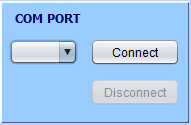
\includegraphics[scale=1]{comport.png}
				\end{center}
			\end{figure}
			\begin{itemize}
				\item Added a panel in Jframe for COM port section and then added jComboBox showing all the available COM ports.
				\item Then added two buttons one to connect to the robot and other to disconnect from the robot.
				\item So after selecting the COM port and clicking on the connect button, the GUI connects to the robot and now reading from the serial port and writing on the serial port is possible
			\end{itemize}
			\item \textbf{Created Buzzer Section in GUI:}
			\begin{figure}[h]
				\begin{center}
					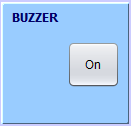
\includegraphics[scale=1]{buzzer.png}
				\end{center}
			\end{figure}
			\begin{itemize}
				\item Created a panel for buzzer section in main JFrame and added a label giving the section title and a button to turn the buzzer on and off in the panel.
				\item To turn on the buzzer "7" or 0x37 is written on the serial port and to turn off the buzzer "9" or 0x39 is written.   
			\end{itemize}   
			\item \textbf{Created Motion Control Section in GUI:}
			\begin{itemize}
				\item Here's the panel added for motion control.\\
				\begin{figure}[h]
					\begin{center}
						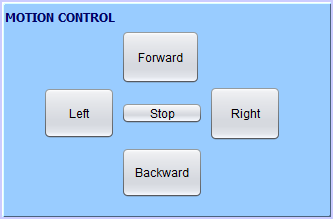
\includegraphics[scale=1]{motioncontrol.png}
					\end{center}
				\end{figure}
				\item  Controls the forward, backward, right, left and stop the motion.
				\item On pressing the forward button "8" which is 0x38 in hex is written on the output stream of serial port and firebird stores this value in UDR2 register and performs the forward action corresponding to that value. 
				\item Similarly for backward motion "2" or 0x32 in hex, for left motion "6" or 0x36 in hex, for right "4" or 0x34 and for stop "5" or 0x35 in hex is written on the output stream of serial port to perform the corresponding action.
			\end{itemize}  
			\newpage    
			\item \textbf{Created Velocity Control Section in GUI:}
			\begin{itemize}
				\item There are two sliders to set the velocity of both left and right motor. After setting the velocity bot will perform the motion with specified velocities.\\
				\begin{figure}[h]
					\begin{center}
						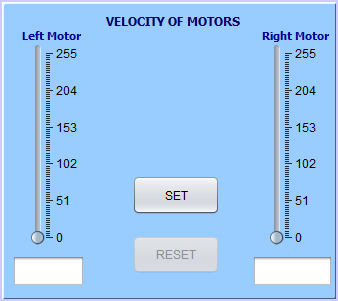
\includegraphics[scale=1]{velocitycontrol.png}
					\end{center}
				\end{figure}
				\item On pressing the set button 0x52, left motor velocity and right motor velocity in hex is written on the output stream of serial port. In the firebird V robot on getting the 0x52 in UDR2 register next two values are stored as left and right velocities.
				\item On clicking the Set button, if both velocities are selected then a dialog box displaying the message that both the velocities have been set will be displayed and if any one velocity is not selected then dialog box showing the message to set the velocities will be displayed.
			\end{itemize} 
			\item \textbf{Created Section for Rotation by some angle and Movement by some Distance in GUI:} \\
			\begin{itemize}
				\item Added panel for Rotation and Movement of the bot and added two text boxes to enter the value of angle and distance and also added button to rotate left and right by that angle and move forward and backward by that distance.
				\newpage
				\begin{figure}[h]
					\begin{center}
						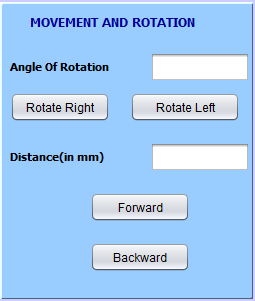
\includegraphics[scale=1]{rotation_movement.png}
					\end{center}
				\end{figure} 
				\item User have to give the angle to rotate it left or right and have to give distance in millimeter to move that distance forward and backward.
				\item To get the value of angle to rotate and distance to move divide the value by 255 and take the mod of value with 255 and send both the value to the bot along with the some hex value which is used to identify which action to perform.
				\item For left rotation 0x57, for right rotation 0x57, for forward movement 0x55 and for backward movement 0x56 is written on the output stream of serial port.
			\end{itemize}   
			\item \textbf{Developed GUI to give the Reading of Sensors: } 
			\begin{itemize}
				\item There are 3 sections of sensors first section for White Line Sensor readings, second section for Distance Sensor readings and third for IR Sensor readings.
				\item  Hex value of ASCII character "T" i.e 0x54 is send to bot to get the reading of all the white line sensors, IR sensors, Distance sensors and battery voltage. On writing the 0x54 on serial port bot sends all the values to the GUI and then GUI displays the sensors reading  using progress bar.
				\item White Line Sensors reading look like this: \\
				\begin{figure}[h]
					\begin{center}
						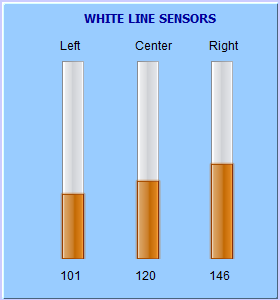
\includegraphics[scale=1]{whitelinesensor.png}
					\end{center}
				\end{figure}
				The White Line Sensors reading varies from 0 to 255 and on white surface sensors give lower reading and on black surface sensors give higher reading.
				\newpage
				\item IR Sensors reading look like this: \\ 
				\begin{figure}[h]
					\begin{center}
						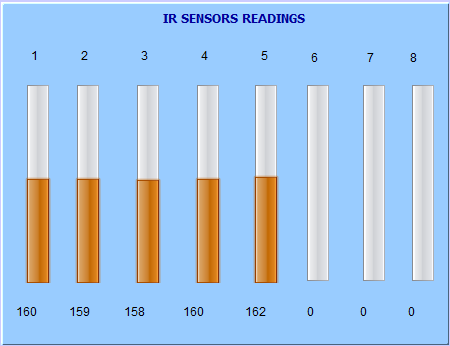
\includegraphics[scale=0.75]{irsensor.png}
					\end{center}
				\end{figure} \\
				IR Sensors 6, 7 and 8 works only when jumper 4 is connected. Sometimes IR sensors reading of 6, 7 and 8 on progress bar does not match the reading on the console. Like reading of these sensors is 0,0,0 on console but on progress bar it shows 90,0,0. IR Sensors reading varies from 0 to 255.
				\newpage
				\item Distance Sensors reading look like this: \\
				\begin{figure}[h]
					\begin{center}
						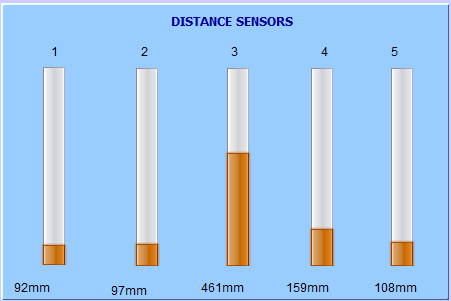
\includegraphics[scale=0.75]{distance_sensor.png}
					\end{center}
				\end{figure} \\
				This is reading when 3rd distance sensor is connected. All other readings are garbage value. Distance Sensors reading varies from 0 mm to 800 mm.
			\end{itemize} 
			\item \textbf{Created Battery Voltage Section in the GUI:}\\
			 This section gives the battery voltage reading. Maximum value of battery voltage is 12V.
			 \begin{figure}[h]
			 	\begin{center}
			 		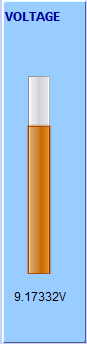
\includegraphics[scale=0.75]{batteryvoltage.png}
			 	\end{center}
			 \end{figure}
			 \item \textbf{Created Section For Servo Motor in GUI:} 
			 \begin{itemize}
			 	\item Added panel in JFrame for servo motors section. There are three sliders and text boxes to set the angle of servo motor to be rotated.
			 	\newpage
			 	\begin{figure}[h]
			 		\begin{center}
			 			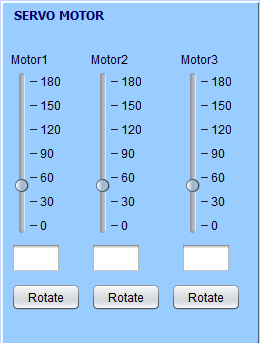
\includegraphics[scale=0.75]{servomotor.png}
			 		\end{center}
			 	\end{figure} 
			 	\item Rotates the Servo Motor S1, S2, S3 by the angle given by user using slider or text box. Servo Motor can rotate form 0 to 180 degrees.
			 	\item Servo motor first goes to its initial position and then rotate to the specified angle.
			 	\item On clicking the rotate button for servo motor 1 0x80 is written on serial port. Similarly 0x 81 for servo motor 2 and 0x82 for servo motor 3 indicating that next value received by the bot is angle to be rotate.
			 	\item Servo Motor should be improved such that it sets the specified angle without going to its initial position. 
			 \end{itemize}
			 \item \textbf{Created Section to Print on LCD in GUI:}
			 \begin{itemize}
			 	\item User can print one character on the LCD by giving the row, column and character to print. \\
			 	\begin{figure}[h]
			 		\begin{center}
			 			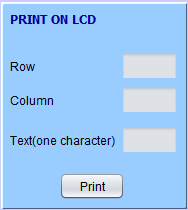
\includegraphics[scale=1]{lcd.png}
			 		\end{center}
			 	\end{figure}
			 	\item On clicking the print button sends 0x83 to identify that next three values which the bot gets are row, column and text to be printed on LCD. 
			 \end{itemize}
			 \newpage 
		   	 \item \textbf{Created Section for Bar Graph LED in GUI:} 
		   	 \begin{itemize}
		   	 	\item User can glow Bar Graph LED by giving the LED number. On clicking the glow button 0x84 is written on the serial port to identify next value which is written is the LED to glow.\\
		   	 	\begin{figure}[h]
		   	 		\begin{center}
		   	 			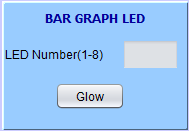
\includegraphics[scale=1]{bargraphled.png}
		   	 		\end{center}
		   	 	\end{figure}
		   	 \end{itemize} 
			 \item This is how final GUI looks like- \\
			 \begin{figure}[h]
				\begin{center}
					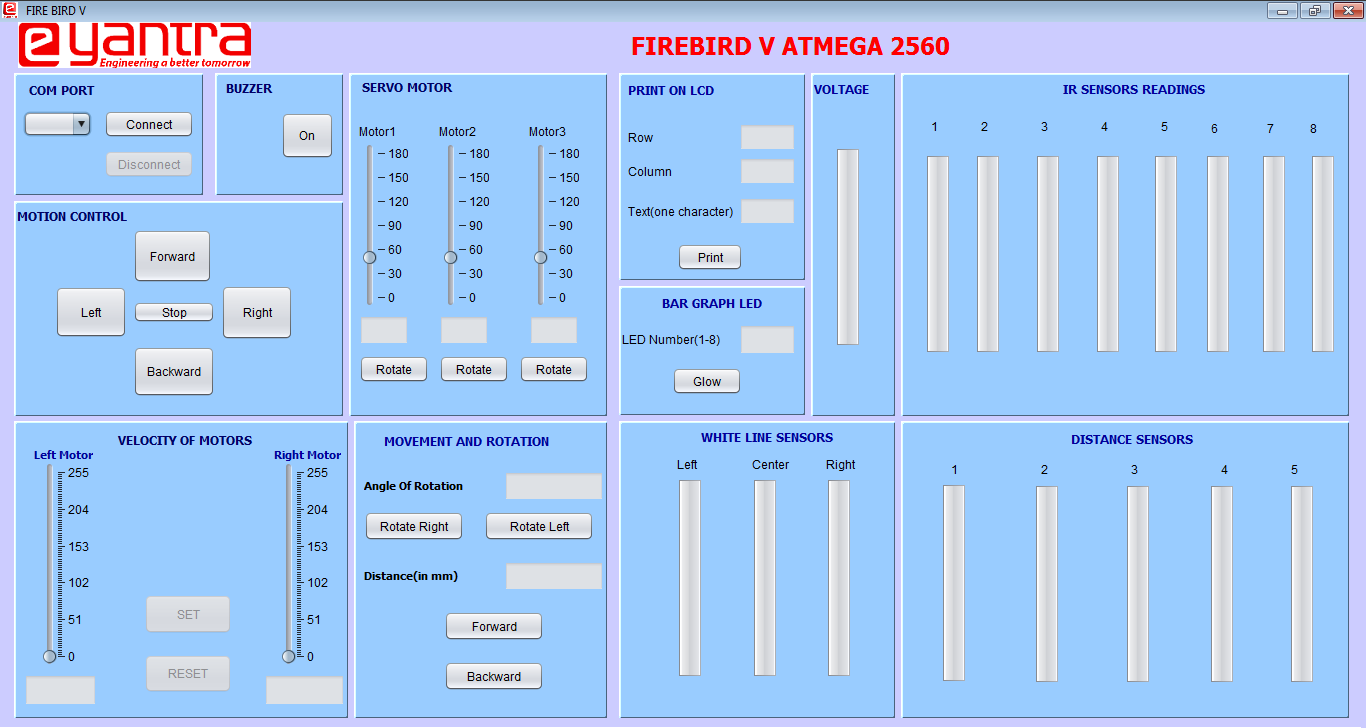
\includegraphics[scale=0.50]{GUI.png}
				\end{center}
			 \end{figure}
			 Using various sections of this GUI test all the components of Firebird V robot.  
		\end{itemize}
		\item \textbf{\large Creating Executable File and Running the GUI on Different Systems:} \\
		\begin{itemize}
			\item Currently we can run the .jar file in command prompt and explicitly copying the rxtxSerial.dll file. Copy rxtxSerail.dll in \%JAVAHOME\% jdk/jre/bin. And then give the command "java -jar filename.jar" in command prompt.
			\item The GUI is running on 32-bit and 64-bit windows 7, Linux and Windows 8.1 OS. Testing the GUI Mac is remaining.
			\item RxTx Library is not supported in Windows 8 OS.
			\item Making a executable file is remaining.
		\end{itemize} 
		\item \large \textbf{Pending Tasks:}
		\begin{itemize}
			\item Interfacing Camera and displaying the output on GUI.
			\item Serial Terminal, Creating CSV file of Input/Output values. 
		\end{itemize}
	\end{enumerate} 
	\newpage
	\textbf{\huge Results and Discussion:} \vspace{1cm} \\
	 The GUI is developed using JAVA to make it platform independent so that it can run on all the operating system and can be used to test all the components of Firebird V robot. The Serial Communication in this done through rxtx library. This library is most suitable as it licenced so its API won't change but its drawback is it is currently not support in windows 8 but updated version of this library will be support in windows 8. The GUI tests the buzzer, LCD, Position Encoders, DC Motors Bar Graph LED, Servo Motors, White Line Sensors, Distance Sensors, IR Sensors and Battery Voltage. \vspace{1cm} \\  
	 \underline{Scope of Improvement/ Future Work:}
	 \begin{itemize}
	 	\item Print string consisting of more than one character on LCD. 
	 	\item Make a separate tab in GUI window which will be like the terminal window where whatever we read from the input stream and whatever we write on the outputstream of serial port is displayed.
	 	\item There can be a separate tab for camera interfacing in GUI. So that user can test the camera on robot.
	 	\item Display a button pressed and button released message on pressing and releasing the boot switch.
	 	\item A installer of the GUI should be made which will be better so that user does not have to install any external library explicitly.  
	 \end{itemize} 
	\newpage
	\textbf{\huge Issues:} \\ \\
	\begin{enumerate}
		\item Reading of Sensors are not always perfect, it sometimes give absurd reading on GUI but correct reading on console.
		\item Text boxes are taking values which are not acceptable. Like text boxes should not accept the values which are not range, also text boxes which requires only numerical value should not accept any other character
		\item Frame does not adapt to different resolutions of the screen. 
	\end{enumerate}
	\newpage
	\textbf{\huge References:} \\ \vspace{1cm}
	\begin{enumerate}
		\item http://www.javatpoint.com/java-tutorial
		\item http://docs.oracle.com/
		\item StackOverflow
		\item https://embeddedfreak.wordpress.com/java-serial-port-trail/
		\item http://rxtx.qbang.org/
	\end{enumerate}
\end{document}